\chapter{Implémentation du M2}

Pour aborder cette 1\up{ère} étape du projet, il est nécessaire de s'appuyer sur les définitions

\begin{description}
\item[Granularité et fort couplage] \hfill \\
  Mélanges de classes de dépendances.
\item[Passage à l'échelle] \hfill \\
  Au bout d'un grand nombre de classe l'évolution et l'extension se voient limitées.
\end{description}


blahblahblahblahblahblahblahblahblah

blahblahblahblahblahblahblahblahblah
\begin{figure}[htb]
%\centering
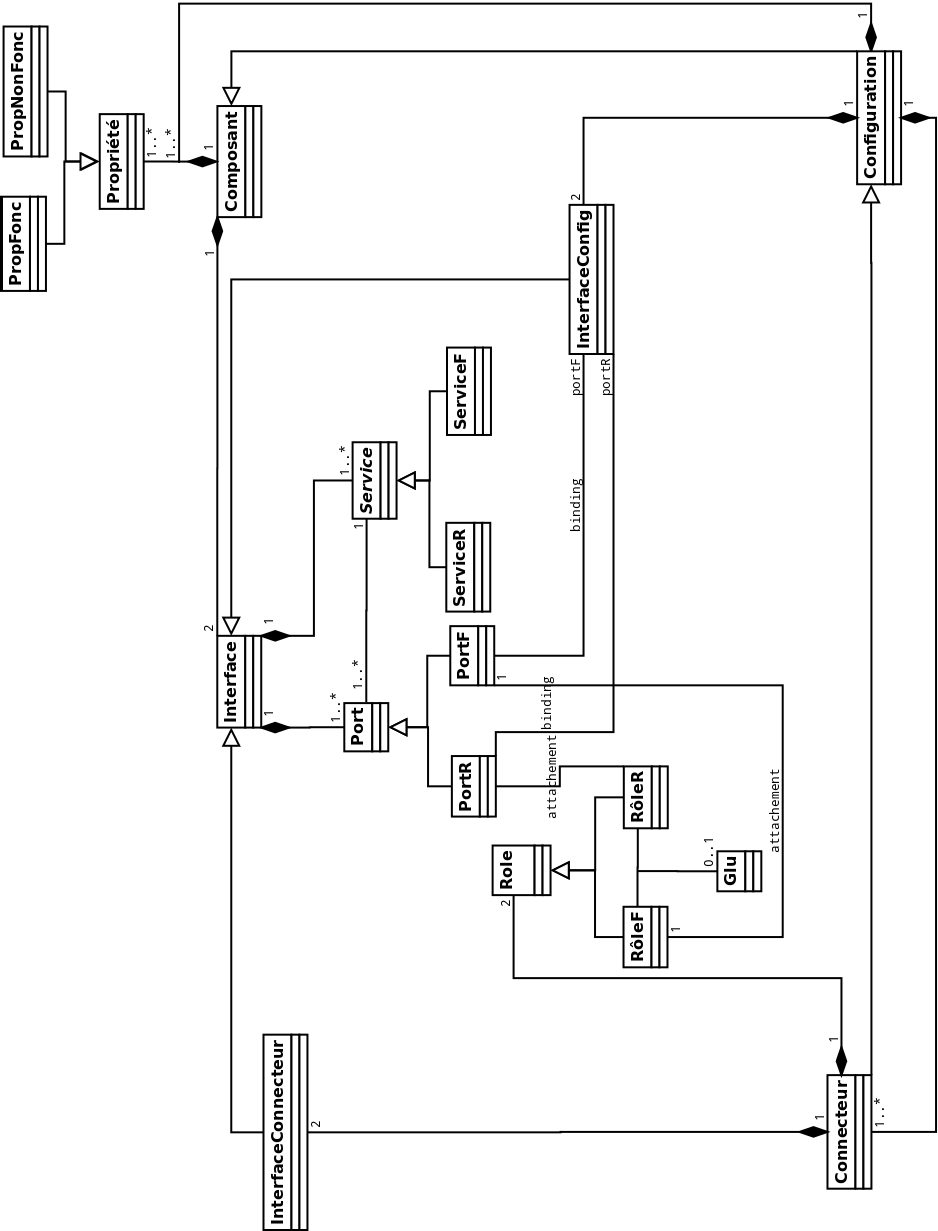
\includegraphics[scale=0.31]{img/M2}
\end{figure}
